% Imported from topics/video-generation/seedance-2.5/reference-timeline.md
\chapter{多参考绑定与时间控制}\label{seedance-m16}
\moduleinfo{M16}{候选设计与工程选型；组合效果待验证}{\hyperref[src-alchemint]{\texttt{alchemint}}、\hyperref[src-phantom]{\texttt{phantom}}、\hyperref[src-ltx-2]{\texttt{ltx-2}}、\hyperref[src-vace]{\texttt{vace}}}

上一章给出参考路径，这里继续展开参考内部的主体归属和时间条件。

多参考继续往下看，文件数量只是表面。两张图可能是同一人的不同角度，也可能是两个相似的人；动作视频里有背景，但目标只需要动作；人物还可能只在第十到十五秒出现。于是参考内容之外，还要同时给出归属和时间，模型才知道每项信息应该用到哪里。

下面以联合音视频主干写一套候选接口，把主体参考和时间控制接起来。参数与预算用于明确计算关系，尚未通过训练验证，不把它们当成已经测得的配置。

\section{一份参考先拆成三个对象}\label{seedance-m16-ux4e00ux4efdux53c2ux8003ux5148ux62c6ux6210ux4e09ux4e2aux5bf9ux8c61}

第一层是原始资产，例如图片、视频或音频。第二层是主体，例如 \codepath{actor_a}、\codepath{car_b}、\codepath{speaker_a}。第三层是绑定规则，说明资产为哪个主体、哪个镜头、哪段时间提供哪类信息。

\begin{verbatim}
{
  "asset_id": "portrait_a_front",
  "subject_id": "actor_a",
  "role": "identity",
  "shot_ids": ["shot_2"],
  "active_intervals_seconds": [[10, 15]],
  "priority": 1
}
\end{verbatim}

\codepath{asset_id} 用来区分文件，\codepath{subject_id} 用来合并同一人的多张视图，\codepath{role} 用来限制应当继承的属性。声音与人物之间另用 speaker-to-subject 映射，不能假设第一段音频必然属于第一张图片。

时间也不能只保留首次和末次出现。人物出现、离开、又回来，中间有一段明确缺席；若直接取两端，就会把缺席也填成出场。因此这里保留区间列表。

\section{描述词与图像为什么需要相同绑定}\label{seedance-m16-ux63cfux8ff0ux8bcdux4e0eux56feux50cfux4e3aux4ec0ux4e48ux9700ux8981ux76f8ux540cux7ed1ux5b9a}

文本绑定的原因可以从两个男人的例子看出来。只写“男人转身”，没有说明是哪一个；若角色描述和对应图片使用同一个索引或角色表示，两个条件就有了共同指向，身份串用的问题才有可监督的对象。

\begin{figure}
\centering
\pandocbounded{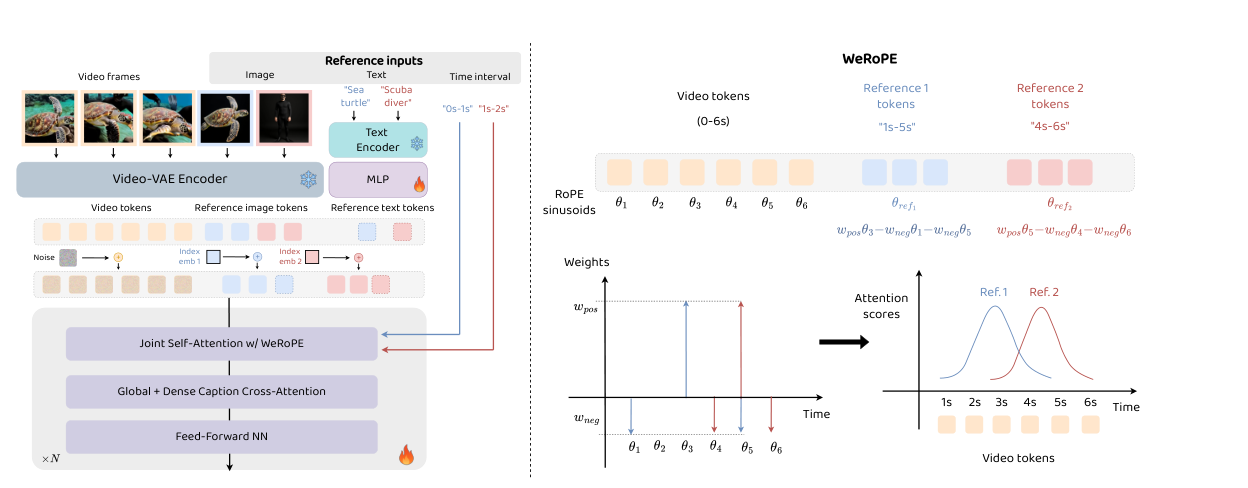
\includegraphics[keepaspectratio,alt={参考图、主体描述与时间区间共同进入模型 （论文示意，来源：alchemint）}]{assets/seedance/figures/timed-reference.png}}
\caption{参考图、主体描述与时间区间共同进入模型 （论文示意，来源：alchemint）}
\end{figure}

图里因此不只放参考图，还放实体词和区间。描述词与图像由同一索引关联，时间再决定它们何时与视频 token 交互。仅在长提示里重复角色名字，并没有显式提供这种内容、归属与时间的对应。

但归属 embedding 仍只是标签。标签告诉模型这些特征属于同一人，脸和服装长什么样还得由图像提供。若素材没有相应外观信息，增加角色标签也不能把它补回来。

\section{三种模态分别怎样编码}\label{seedance-m16-ux4e09ux79cdux6a21ux6001ux5206ux522bux600eux6837ux7f16ux7801}

{\def\LTcaptype{table} % do not increment counter
\small\setlength{\tabcolsep}{3pt}\renewcommand{\arraystretch}{1.18}
\begin{longtable}[]{@{}
  >{\raggedright\arraybackslash}p{(\linewidth - 4\tabcolsep) * \real{0.1900}}
  >{\raggedright\arraybackslash}p{(\linewidth - 4\tabcolsep) * \real{0.3900}}
  >{\raggedright\arraybackslash}p{(\linewidth - 4\tabcolsep) * \real{0.4200}}@{}}
\toprule\noalign{}
\begin{minipage}[b]{\linewidth}\raggedright
输入
\end{minipage} & \begin{minipage}[b]{\linewidth}\raggedright
内容路径
\end{minipage} & \begin{minipage}[b]{\linewidth}\raggedright
需要分开的角色信息
\end{minipage} \\
\midrule\noalign{}
\endhead
\bottomrule\noalign{}
\endlastfoot
图片 & 与目标视频相同的 VAE、空间投影、主体 crop & 身份、服装、场景、风格 \\
视频 & VAE 时空特征；额外提取 pose、flow、相机轨迹 & 动作与相机不能默认继承人物身份 \\
音频 & 同一音频 VAE 的时序特征、说话人分段与文字转录 & 音色、节奏、对白内容、音乐 \\
\end{longtable}
}

图片与视频先使用同一个视觉潜空间，避免又引入一套没有对齐的像素表示。不过每份素材要独立编码：不连续视频若先在像素时间轴拼接，因果 VAE 会把前一份素材当作后一份的历史，边界关系已经变了。

只借动作时，可以优先送姿态、光流和相机条件，关闭不需要的外观 token。音频也一样，一句参考语音可能只提供音色，不是要求输出这句台词。同说话人跨文本配对监督音色，时间对齐文字与波形监督逐字对白，两者的数据定义不同。

音色和风格可以压成摘要，精确对白、节拍或已有配乐则不能只靠32个摘要token承载。需要保持原声音和时序时，使用对齐到目标媒体时钟的完整干净音频条件，输出复用原波形；对应约25Hz的条件序列单独计入计算预算。这样要与``只借音色、生成新台词''的任务分开训练。

\section{固定预算怎样保留细节}\label{seedance-m16-ux56faux5b9aux9884ux7b97ux600eux6837ux4fddux7559ux7ec6ux8282}

候选起点为每图 32 个摘要 token、每视频 64 个、每音频 32 个。30 图和 10 视频共 1600 个视觉参考 token，10 音频共 320 个音频参考 token，分别位于 2048 与 512 的预算以内。

这些是\textbf{压缩后的条件预算}，不是原始 VAE 序列长度，也不是已证明充分的容量。先用少量可学习 query 对每份素材独立汇聚：

\[
R_j=\operatorname{Attn}(Q_j^{\mathrm{pool}},K_j^{\mathrm{asset}},V_j^{\mathrm{asset}}).
\]

压缩之前先保留局部结构：图片有 crop 坐标，视频有动作阶段，音频有时间段与 speaker，再加 role、subject 和位置。若先把所有素材平均成一个向量，后面就很难再恢复哪一部分来自哪个人。

读取也按镜头进行。细 logo、纹理或音色在压缩中消失时，应先调整相应主体的预算，或用确定性合成处理交付；继续增加无关镜头的素材，不能恢复已经丢掉的信息。

\section{时间控制放在哪里}\label{seedance-m16-ux65f6ux95f4ux63a7ux5236ux653eux5728ux54eaux91cc}

时间控制可以放进参考位置，也可以放进 cross-attention 的偏置。加权 RoPE 尝试让一个参考在整个区间持续可读，而不只编码区间中点，因此有机会区分长短区间。这里仍是学习型偏置，尚不能从注意力分数直接推出人物一定按时出场。

为降低首版迁移风险，这套候选方案先保留主干原 RoPE，只在新增参考支路增加显式时间门：

\[
g_j(\tau)=\sum_k
\sigma\!\left(\frac{\tau-a_{jk}}{\delta}\right)
\sigma\!\left(\frac{b_{jk}-\tau}{\delta}\right).
\]

区间为 \([a_{jk},b_{jk})\)，\(\delta\) 控制边界过渡。实际将重叠区间合并，并把 \(g_j\) 限制到 \([0,1]\)。对应 attention bias 为：

\[
B_{ij}=\log\bigl(\varepsilon+(1-\varepsilon)g_j(\tau_i)\bigr).
\]

因为 attention 在 softmax 前加上 \(B_{ij}\)，相当于在归一化前将该参考位置的指数权重乘以 \(\varepsilon+(1-\varepsilon)g_j(\tau_i)\)。所以这个时间门是在改变读取权重；它没有直接改写目标人物是否存在，后面的正负时间监督仍然需要。

角色或镜头不相容时，可以把连接直接屏蔽；时间边缘先用软门，留出进入、离开与运动模糊的过渡。还要保留一个始终可读的 null token，否则某行参考全部不可见，softmax 本身就没有定义。

空间query并不天然知道自己属于哪个主体。没有布局、源跟踪或可靠预测区域时，只按镜头允许的主体集合做粗筛，靠共享主体embedding与训练学习对应；有可靠区域时才加入空间约束。训练中若使用真值区域，推理也必须提供相同类型的条件，或在训练时混入预测误差，不能借用目标真值暗中完成绑定。

\section{不能把``看不到参考''当成``角色一定不出现''}\label{seedance-m16-ux4e0dux80fdux628aux770bux4e0dux5230ux53c2ux8003ux5f53ux6210ux89d2ux8272ux4e00ux5b9aux4e0dux51faux73b0}

注意力控制住了参考，是否也就控制住人物出场？还没有。文本或历史仍可能让主干在区间外生成人物。因此训练必须同时有区间内出现、区间外缺席，以及多人重叠的样本，让“什么时候不出现”也进入监督。

可从实体词、检测与分割跟踪提取可见区间，再选与目标相隔较远的主体视图，减少复制。不过没检测到，不一定就是离场，也可能被遮挡，所以标签要保存可见性置信度，不能把所有漏检写成角色不存在。

验收分别统计区间内身份、区间外误出现、边界误差、多人串用、动作跟随和背景泄漏。两图两个角色、相同中点不同区间长度、间断出场和同时出场，都是必须保留的对照。

\section{极简代码与工程入口}\label{seedance-m16-ux6781ux7b80ux4ee3ux7801ux4e0eux5de5ux7a0bux5165ux53e3}

单区间时间 bias 的计算见 \hyperref[code-reference-timing]{reference\_timing.py}，多区间需先按主体合并。参考支路的布尔可读mask见 \hyperref[code-reference-adapter]{reference\_adapter.py}；将时间bias与归属mask合成、添加null token由调用者完成。这些代码只说明机制，未执行。

真实主体参考可从 \href{https://github.com/Phantom-video/Phantom}{Phantom-Wan} 阅读；时间控制方法的 \href{https://snap-research.github.io/Video-AlcheMinT/}{AlcheMinT 项目} 提供论文与展示。本方案采用显式时间门作为首版设计，不将它称为 WeRoPE 原实现，也不声称这些方法已被用于 Seedance 2.5。
